\documentclass{beamer}

\newcommand{\nologo}{\setbeamertemplate{logo}{}} 
\usetheme{Boadilla}
\usepackage{color}
\usepackage{graphicx}
\usepackage[caption = false]{subfig}
\usepackage{float}
\usepackage[english]{babel}
\usepackage{media 9}


%%%%%%%%%%%%%%%%%%%%%%%%%%%%%%%%%%%%%%%%%%%%%%%%%%%%%%%%%%

% Fix the footer

\makeatother
\setbeamertemplate{footline}
{
  \leavevmode%
  \hbox{%
  \begin{beamercolorbox}[wd=0.5\paperwidth,ht=2.25ex,dp=1ex,center]{author in head/foot}%
    \usebeamerfont{author in head/foot}\insertshortauthor
  \end{beamercolorbox}%
  \begin{beamercolorbox}[wd=0.5\paperwidth,ht=2.25ex,dp=1ex,center]{title in head/foot}%
    \usebeamerfont{title in head/foot}\insertshorttitle\hspace*{3em}
    \insertframenumber{} / \inserttotalframenumber\hspace*{1ex}
  \end{beamercolorbox}}%
  \vskip0pt%
}
\makeatletter
\setbeamertemplate{navigation symbols}{}

%%%%%%%%%%%%%%%%%%%%%%%%%%%%%%%%%%%%%%%%%%%%%%%%%%%%%%%%%%


\title{Random Walk, Diffusion, and Cluster Growth}


\author{Connor Hann, Xiaomeng Jia, Peifan Liu and Xinyu Wu}
\institute[] {Physics Department, Duke University}


\pgfdeclareimage[height=0.5cm]{university-logo}{duke_logo}
\logo{\pgfuseimage{university-logo}}

\begin{document}

\begin{frame}
  \titlepage
\end{frame}

\begin{frame}{Outline}
  \tableofcontents
\end{frame}

%%%%%%%%%%%%%%%%%%%%%%%%%%%%%%%%%%%%%%%%%%%%%%%%%%%%%%%%%%

\section{2D Random Walk}

%%%%%%%%%%%%%%%%%%%%%%%%%%%%%%%%%%%%%%%%%%%%%%%%%%%%%%%%%%

\subsection{One-dimensional random walks}

\begin{frame}{1D Random Walk}

RMS distance of an ensemble of random walkers after $n$ steps
\begin{equation}
	\sqrt{<x_n^2>} = \sqrt{\sum\limits_{i=1}^{n}\sum\limits_{j=1}^{n}<\Delta x_i\Delta x_j>} = \sqrt{n}\Delta x
\end{equation} 

Diffusive motion:
\begin{equation}
	<x^2(t)> = 2Dt
\end{equation}
where $D = v\cdot\Delta x/2 = (\Delta x)^2/(2\Delta t)$ is the diffusion constant.

\end{frame}

\subsection{Two-dimensional random walks}

\begin{frame}{2D Random Walk (1)}

Diffusive motion:
\begin{equation}
	<r^2(t)> = 2Dt
\end{equation}
Where $D = (\Delta x)^2/(4\Delta t)$.
	
\begin{figure}[H]
	\centering
	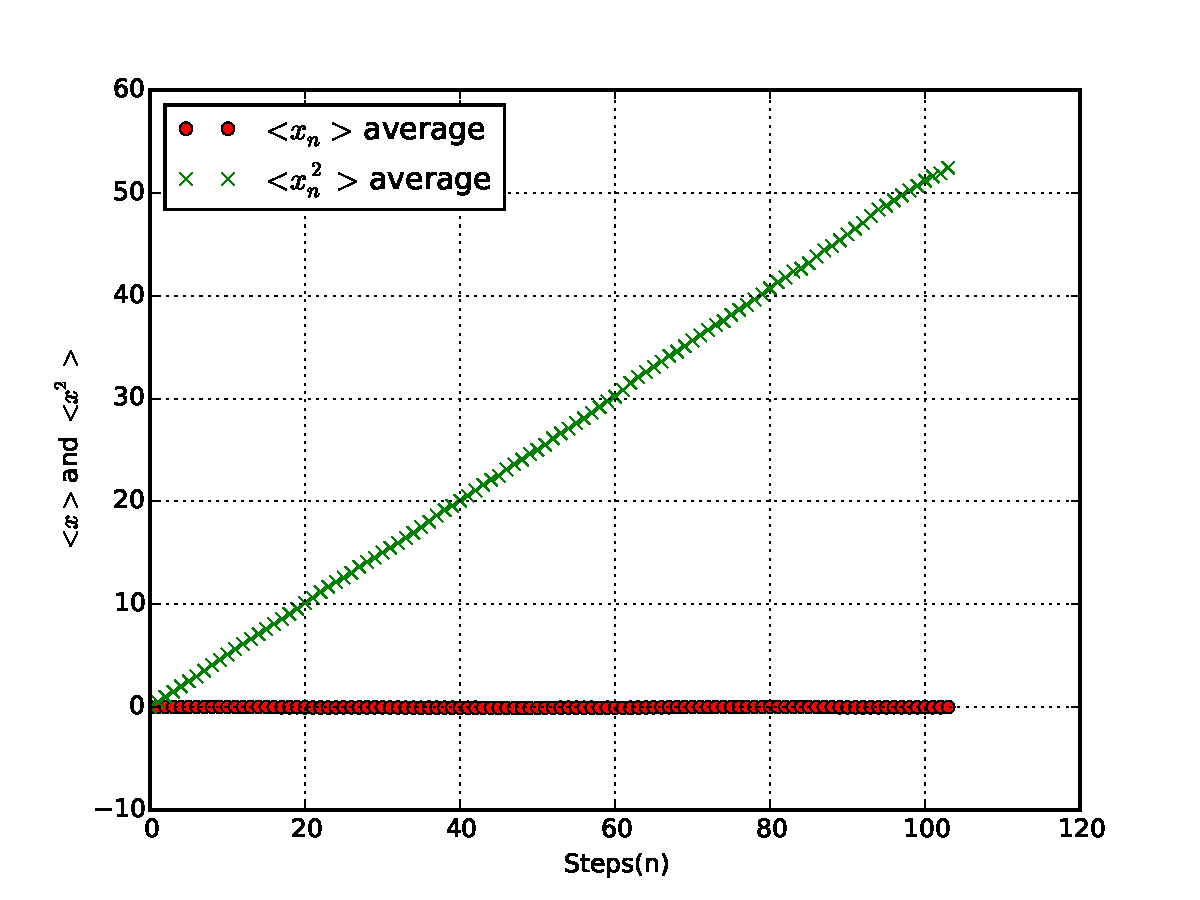
\includegraphics[width=0.7\textwidth]{rwxn.pdf}
	%\caption{$ <x(t)> $ and  $ <x^2(t)> $ in 1D random walking, averaging over a 10000 random walker ensemble.}
\end{figure}
	

\end{frame}

\begin{frame}{2D Random Walk (2)}

\begin{figure}[H]
	\centering
	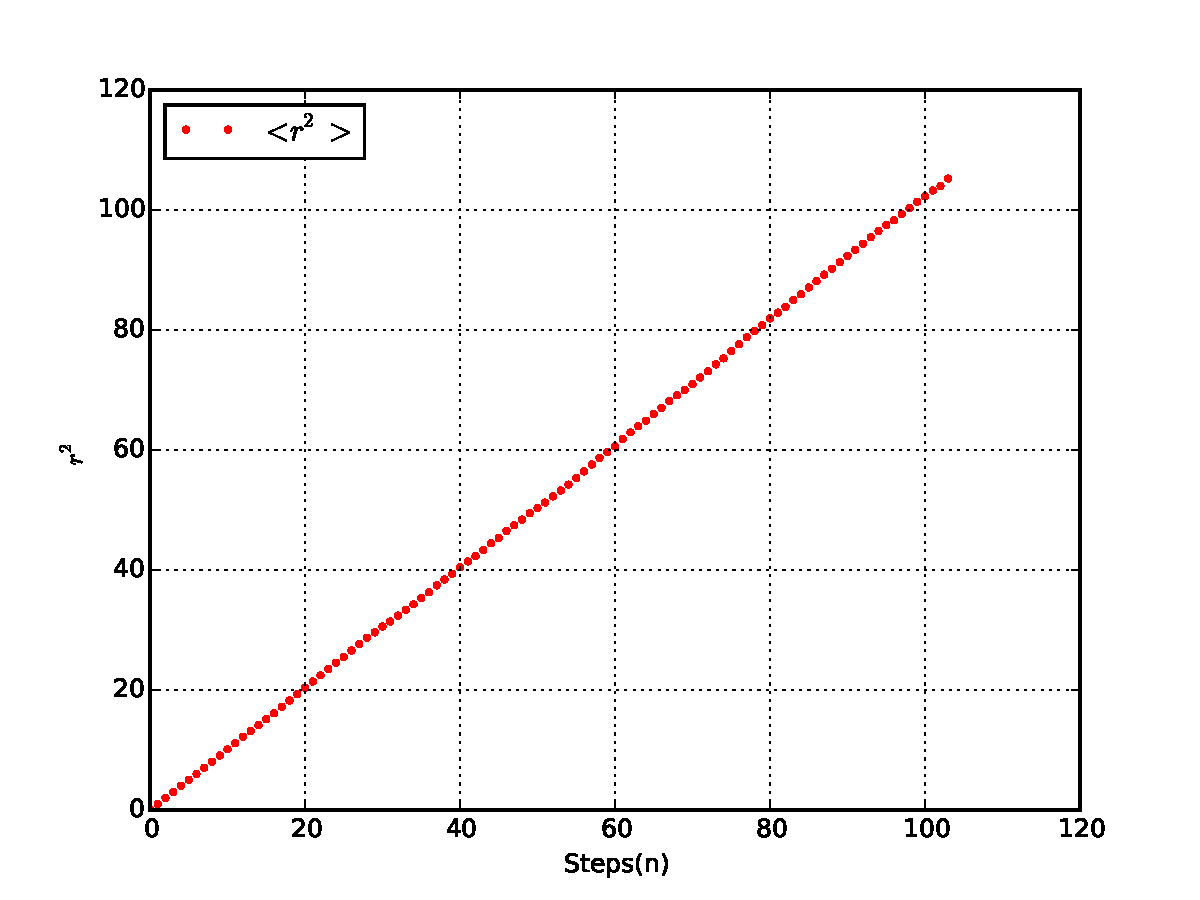
\includegraphics[width=0.5\textwidth]{rwxn2.pdf}
  	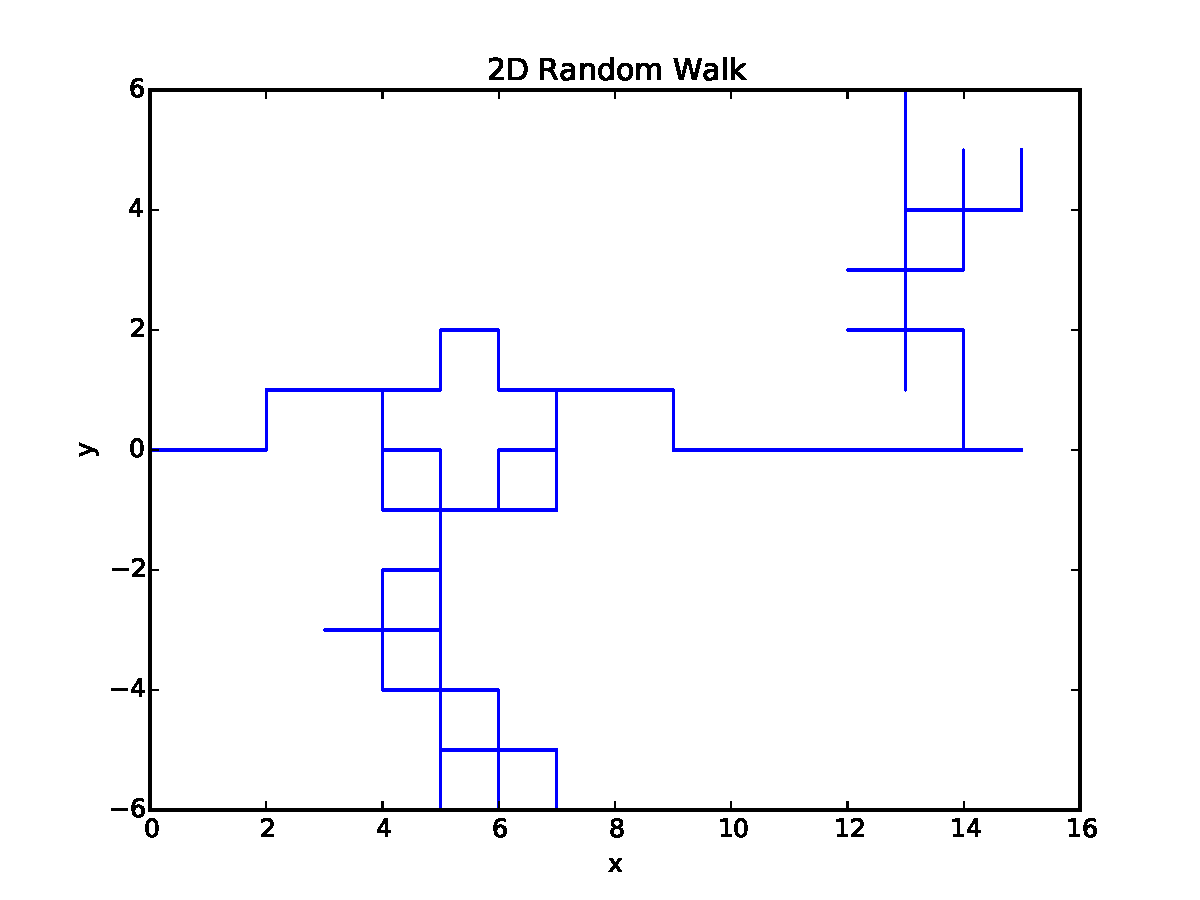
\includegraphics[width=0.5\textwidth]{rwxn3.pdf}
\end{figure}
	

\end{frame}

%%%%%%%%%%%%%%%%%%%%%%%%%%%%%%%%%%%%%%%%%%%%%%%%%%%%%%%%%

\section{Diffusion}

%%%%%%%%%%%%%%%%%%%%%%%%%%%%%%%%%%%%%%%%%%%%%%%%%%%%%%%%%

\subsection{Mathematical background}

\begin{frame}{Diffusion}
\quad Diffusion equation
\begin{equation}
\frac{\partial\rho}{\partial t}=D\nabla^2\rho
\end{equation}
\quad discretize $t=k\Delta t, x=i\Delta x$,
\begin{equation}
\rho_{i,k+1}=\rho_{i,k}+D\frac{\Delta t}{\Delta x^2}(\rho_{i+1,k}+\rho_{i-1,k}-2\rho_{i,k})
\end{equation}
\quad \quad with $\Delta t<\frac{\Delta x^2}{2D}$
\end{frame}

\begin{frame}{Normal Distribution}

One-dimensional normal distribution
\begin{equation}
	\rho(x,t) = \frac{1}{\sqrt{2 \pi \, \sigma(t)^2}} \, \text{exp} \left( - \frac{x^2}{2\sigma(t)^2} \right)
\end{equation}

\begin{equation}
\langle x^2\rangle=\int_{-\infty}^{\infty}\frac{1}{\sqrt{2\pi}\sigma(t)}x^2exp(-\frac{x^2}{2\sigma(t)^2})=\sigma(t)^2
\end{equation}
\end{frame}

\begin{frame}{Animation}
\begin{center}
\includemedia[
    activate=onclick,
    width=0.75\textwidth
]{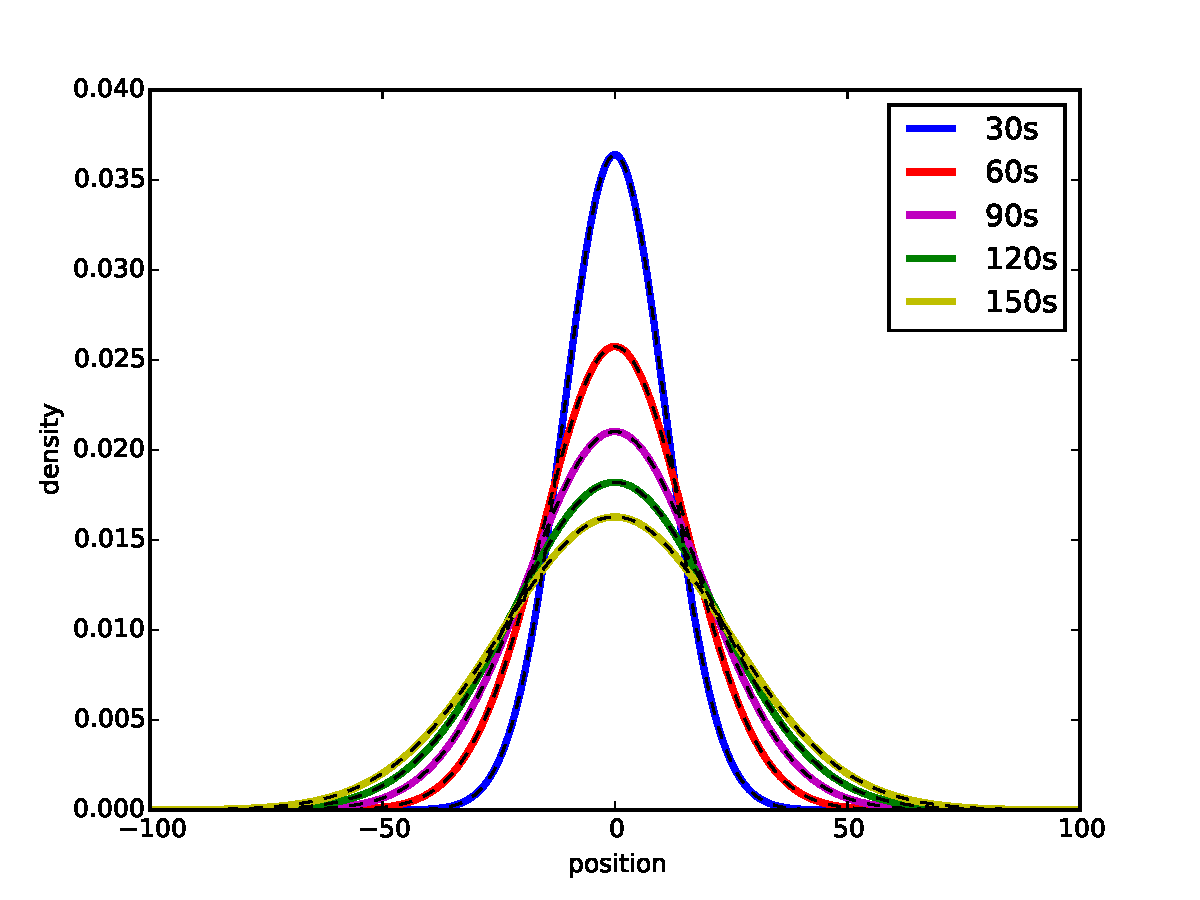
\includegraphics{diffusion.png}}{diffusion.swf}
\end{center}
\end{frame}

\subsection{Numerical results}

\begin{frame}{Diffusion time dependence}

\begin{figure}[H]
	\centering
	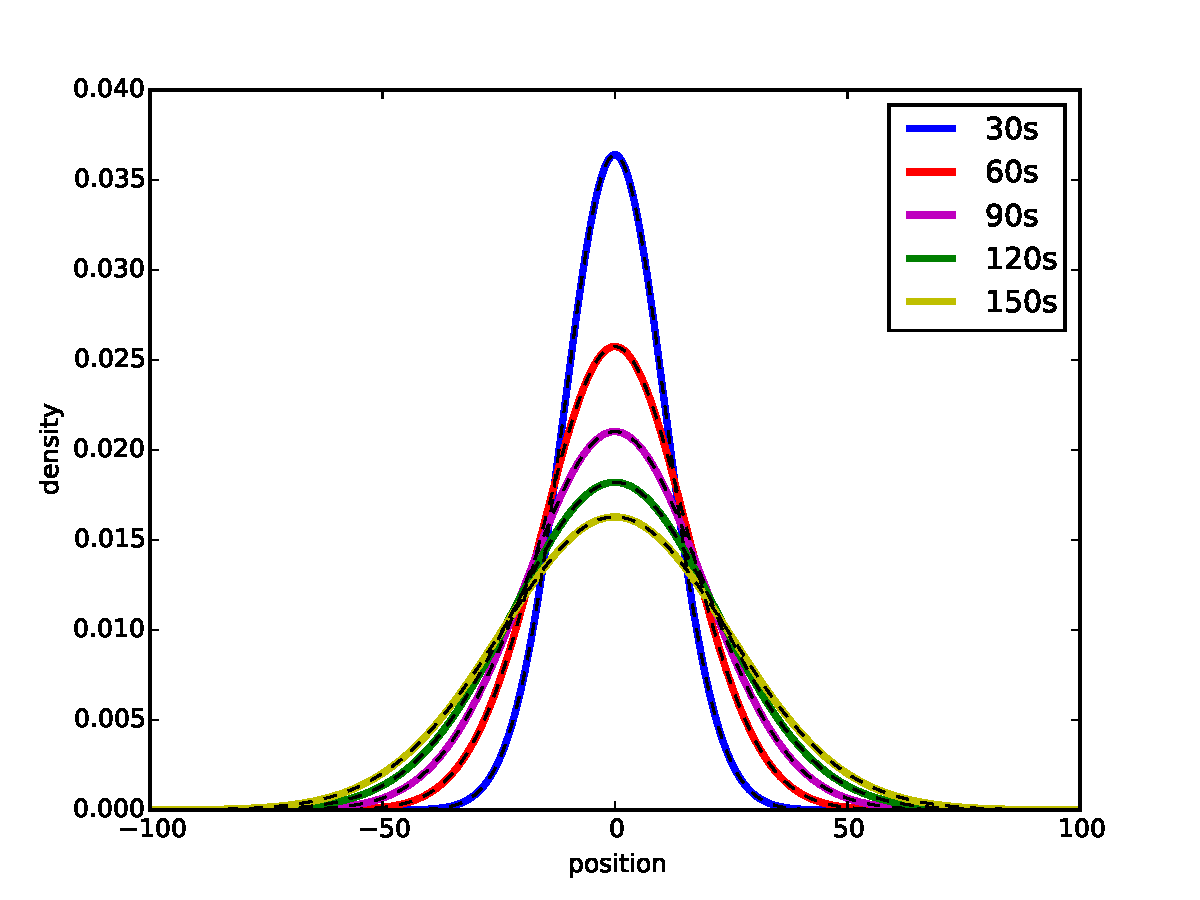
\includegraphics[width=0.8\textwidth]{diffusion.pdf}
\end{figure}
\begin{equation*}
\langle x^2\rangle=\sigma(t)^2=2Dt
\end{equation*}

\end{frame}

%%%%%%%%%%%%%%%%%%%%%%%%%%%%%%%%%%%%%%%%%%%%%%%%%%%%%%%%%

\section{Crystal Growth}

%%%%%%%%%%%%%%%%%%%%%%%%%%%%%%%%%%%%%%%%%%%%%%%%%%%%%%%%%

\subsection{Background}

\begin{frame}{Crystal Growth with Diffusion Limited Aggregation (DLA)}

DLA Algorithm:

\begin{enumerate}

\item Consider a lattice of points with a seed particle at the origin

\item Release a particle from a random location a distance $R$ from the origin

\item Let the particle perform a random walk until it hits the perimeter of the cluster or strays too far

\item Repeat until the cluster reaches the edge of the circle(Radius=100)

\end{enumerate}

\textcolor{red}{Animation}
\end{frame}

\begin{frame}{Example DLA cluster}

\begin{figure}[H]
	\centering
	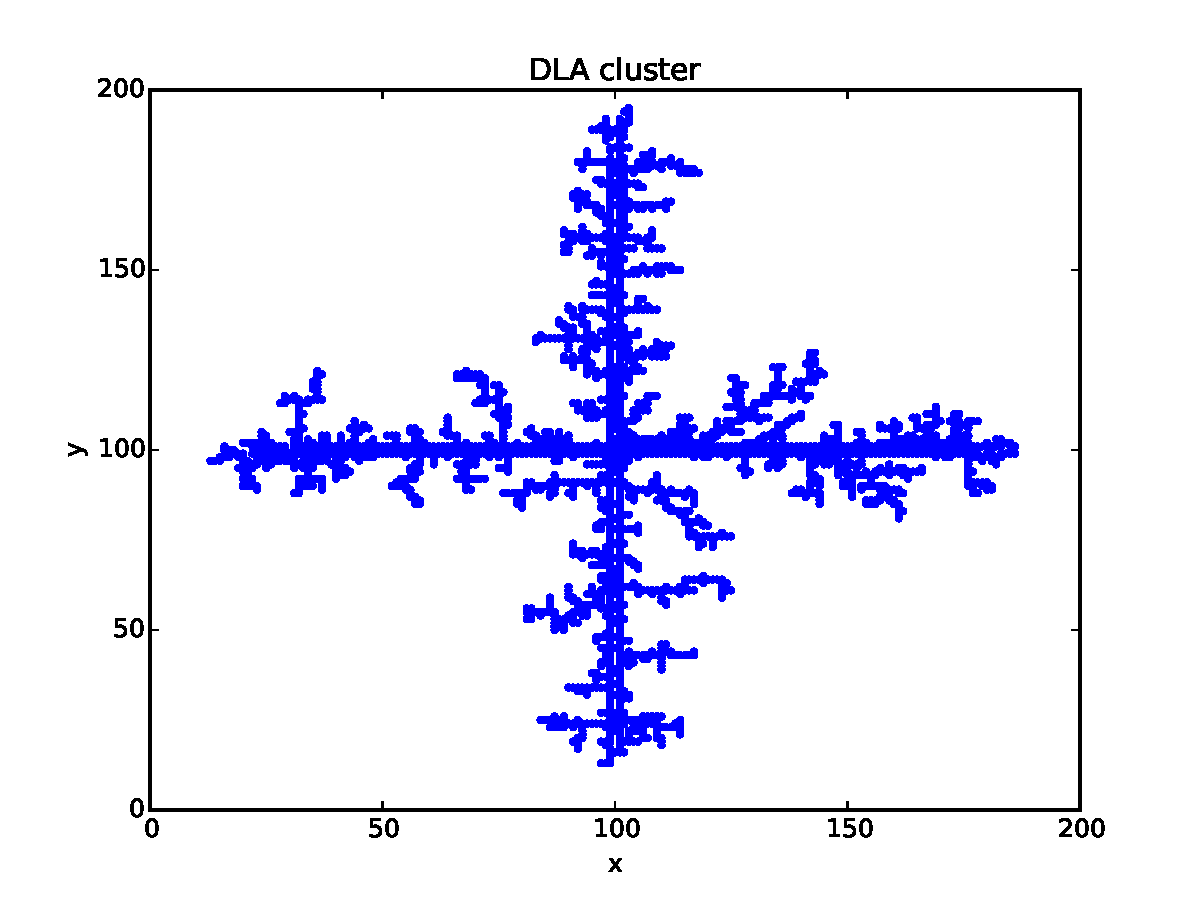
\includegraphics[width=0.8\textwidth]{dla.pdf}
\end{figure}

\end{frame}

\begin{frame}{Typical clusters}

\begin{figure}[H]
	\centering
	\subfloat{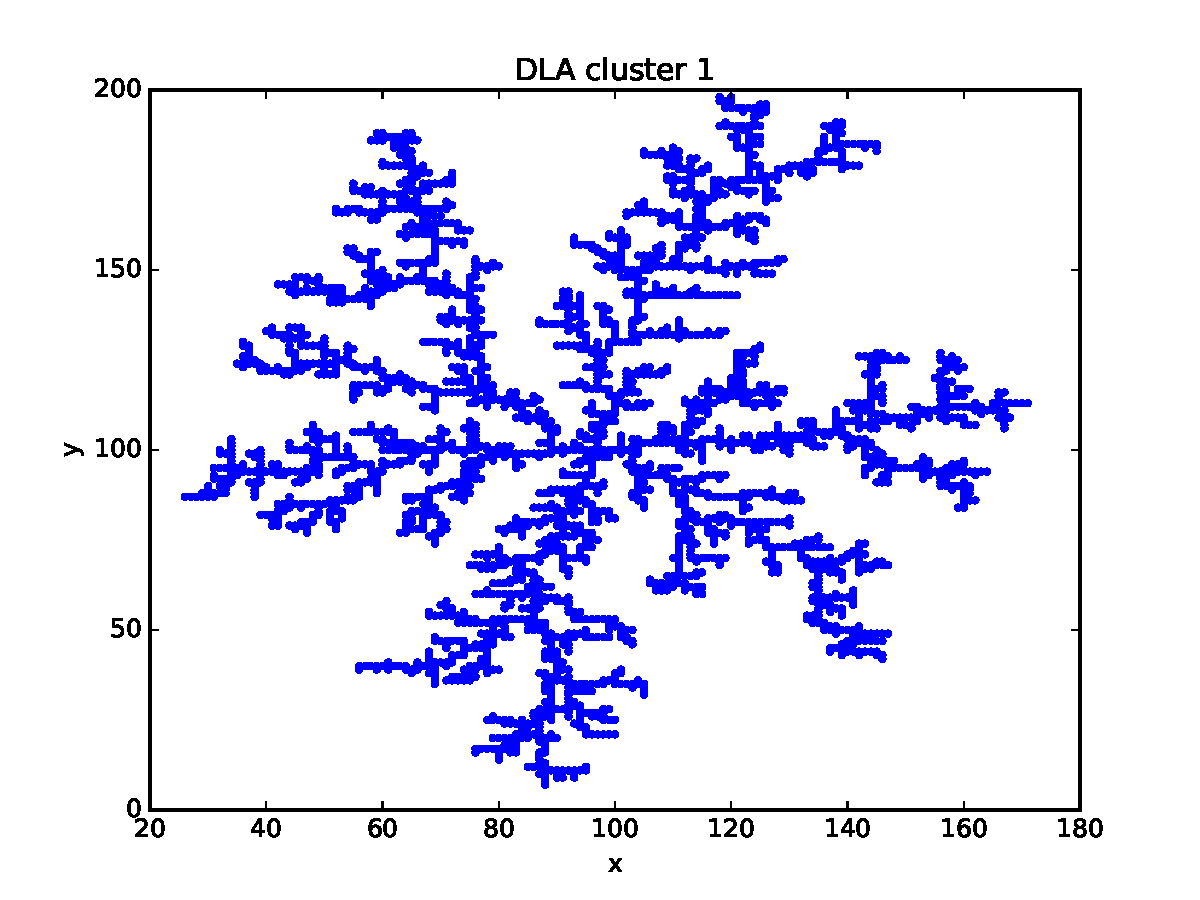
\includegraphics[width = 0.4\textwidth]{dla_0}}
	\subfloat{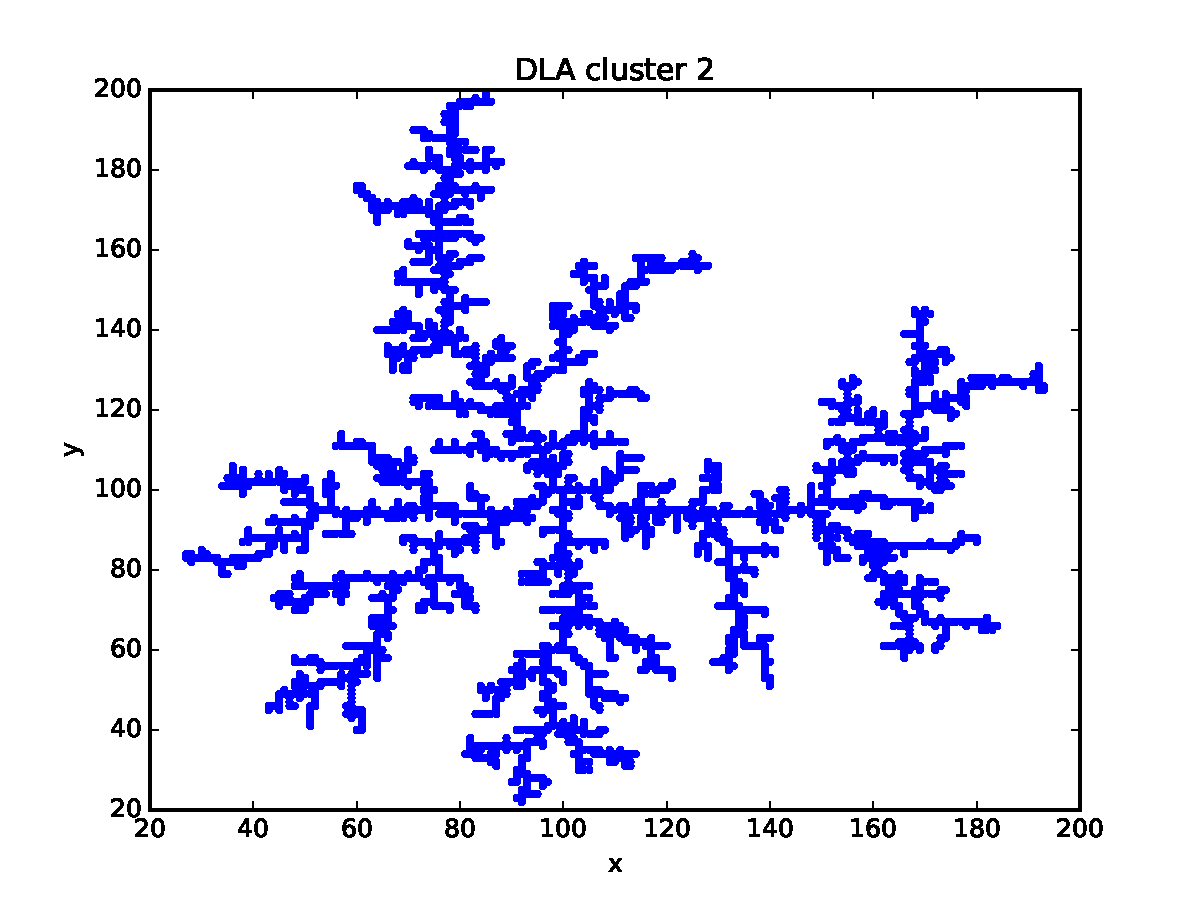
\includegraphics[width = 0.4\textwidth]{dla_1}}\\
	\subfloat{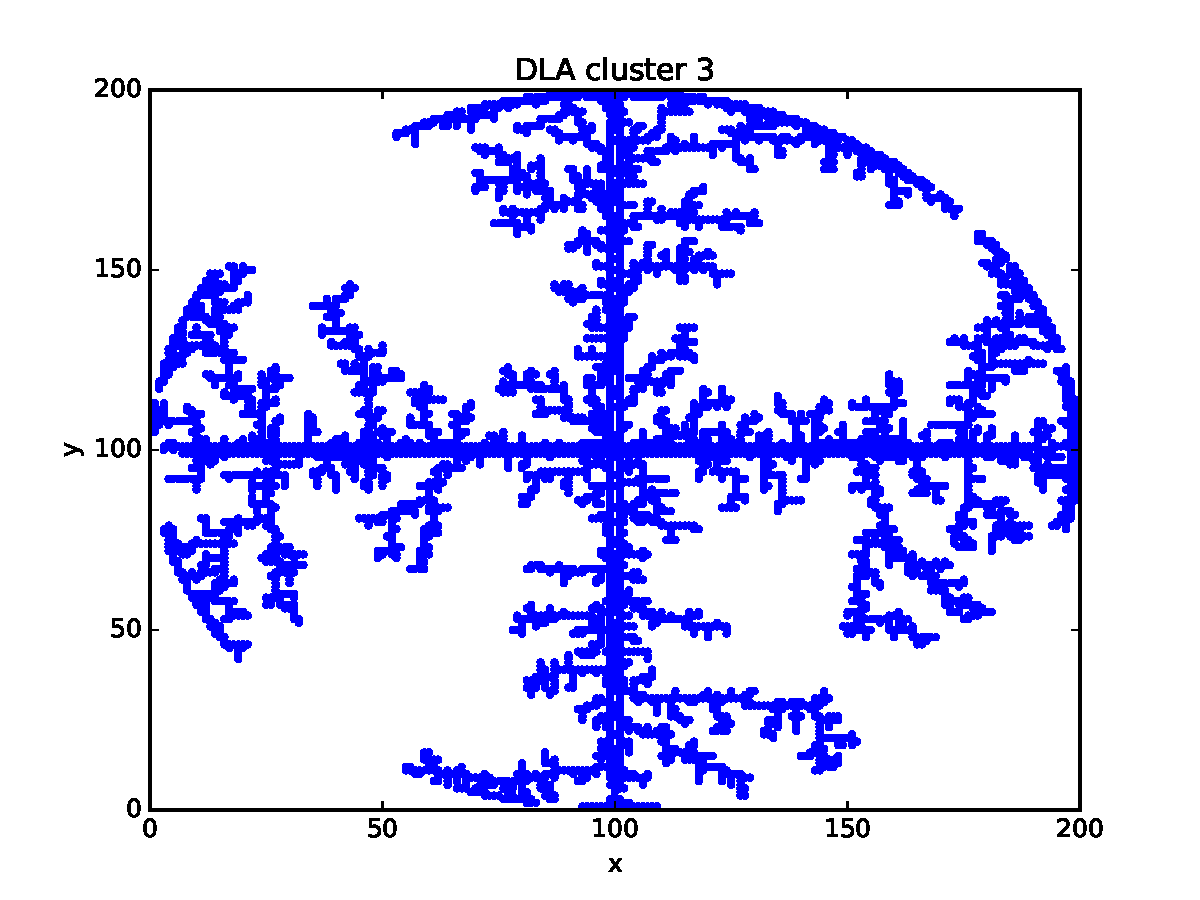
\includegraphics[width = 0.4\textwidth]{dla_2}}
	\subfloat{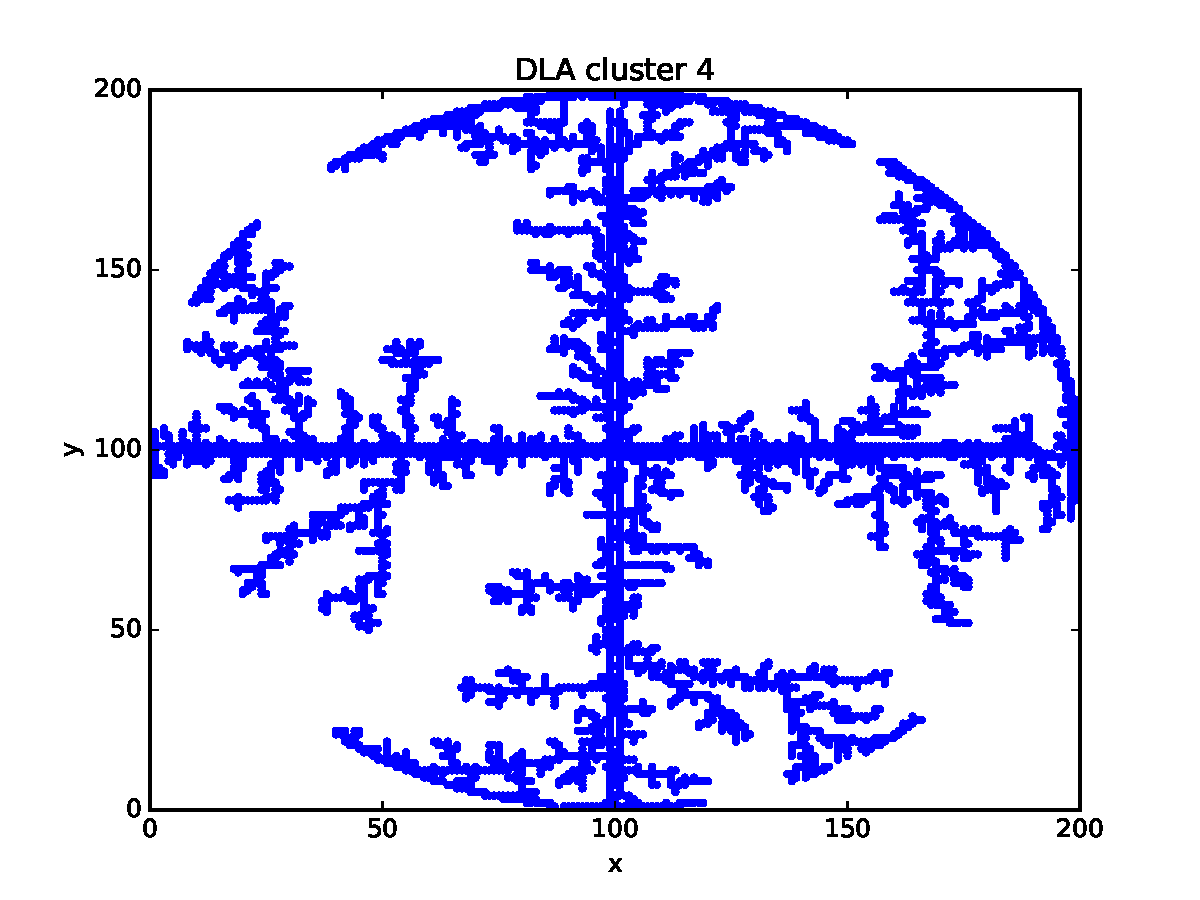
\includegraphics[width = 0.4\textwidth]{dla_3}} 
\end{figure}

\end{frame}

\subsection{Fractal Dimension}

\begin{frame}{Fractal Dimension $d_f$ (1)}

\begin{figure}[H]
	\centering
	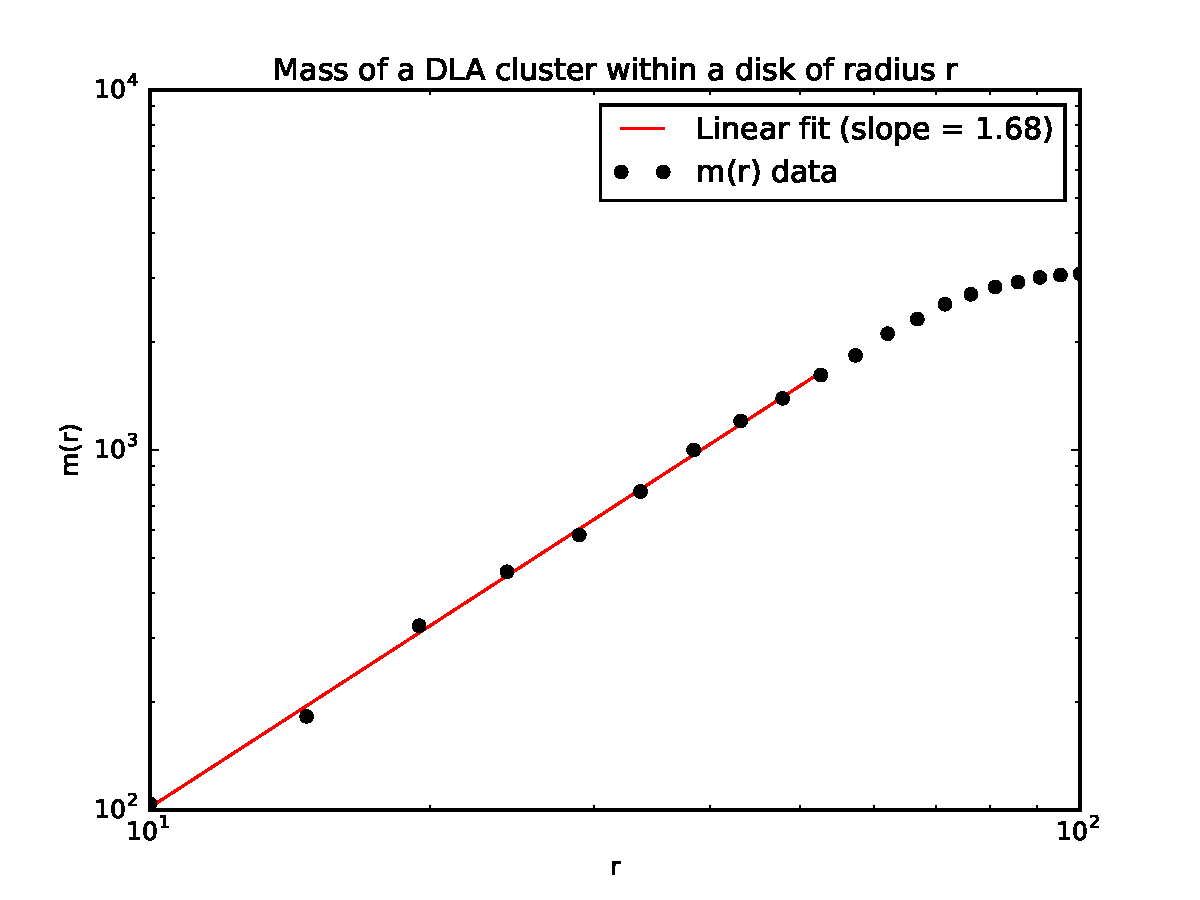
\includegraphics[width=0.7\textwidth]{mass_vs_R.pdf}
\end{figure}

\end{frame}

\begin{frame}{Fractal Dimension $d_f$ (2)}


\begin{center}
\small
\begin{tabular}{ |c|c|c|c|c|c|c|c|c|c|c| } 
 \hline
Cluster & 1 & 2 & 3 & 4 & 5 & 6 & 7 & 8 & 9 & 10 \\ 
\hline
 $d_f$& 1.74 & 1.63 & 1.77 & 1.55 & 1.66 & 1.58 & 1.64 & 1.74 & 1.74 & 1.75 \\ 
 \hline
\end{tabular}
\end{center}

Average value over 10 runs: $d_f = 1.68(07)$\\
Expected value: $d_f  = 1.65$

\end{frame}

%%%%%%%%%%%%%%%%%%%%%%%%%%%%%%%%%%%%%%%%%%%%%%%%%%%%%%%%%
%%%%%%%%%%%%%%%%%%%%%%%%%%%%%%%%%%%%%%%%%%%%%%%%%%%%%%%%%
%%%%%%%%%%%%%%%%%%%%%%%%%%%%%%%%%%%%%%%%%%%%%%%%%%%%%%%%%

%\begin{thebibliography}{99}

% e.g.
%\bibitem{ref:Johnson28}
%J.~B.~Johnson, Phy. Rev. 32, 1 (1928).

%\end{thebibliography}


\end{document}


